\documentclass[xcolor=x11names,compress]{beamer}

%% General document %%%%%%%%%%%%%%%%%%%%%%%%%%%%%%%%%%
\usepackage{graphicx}
\graphicspath{{graphics/}}
\usepackage{animate}
\usepackage{tikz}

% ########For highlight boxes over equations########
\usepackage{color}
\input{inputs/rgb}
\definecolor{capri}{rgb}{0,.75,1}
\definecolor{coral}{rgb}{1,.2,.2}
\newcommand{\hltyellow}[1]{\colorbox{yellow}{$\displaystyle #1$}}
\newcommand{\hltblue}[1]{\colorbox{capri}{$\displaystyle #1$}}
\newcommand{\hltred}[1]{\colorbox{coral}{$\displaystyle #1$}}
\newcommand{\hltgreen}[1]{\colorbox{green}{$\displaystyle #1$}}

\usepackage{ulem}
\renewcommand<>{\sout}[1]{
  \only#2{\beameroriginal{\sout}{#1}}
  \invisible#2{#1}
}

%%%%%%%%%%%%%%%%%%%%%%%%%%%%%%%%%%%%%%%%%%%%%%%%%%%%%%

%% Beamer Layout %%%%%%%%%%%%%%%%%%%%%%%%%%%%%%%%%%

\usetheme{Madrid}
\usecolortheme{seahorse}
\setbeamertemplate{headline}{}

\usepackage{pdfpages}

% ###Comment/Uncomment to display/hide navigation symbols at bottom:
\setbeamertemplate{navigation symbols}{}

% ###Comment/Uncomment to hide/display outline at top:
% \useoutertheme[subsection=false,shadow]{miniframes}

% \useinnertheme{default}

\setbeamertemplate{footline}
{
  \leavevmode%
  \hbox{
  \begin{beamercolorbox}[wd=.1\paperwidth,ht=2.2ex,dp=1ex,center]{author in head/foot}
    \usebeamerfont{author in head/foot}\insertshortauthor
  \end{beamercolorbox}
  \begin{beamercolorbox}[wd=.8\paperwidth,ht=2.2ex,dp=1ex,center]{title in head/foot}%
    \usebeamerfont{title in head/foot}\insertshorttitle\hspace*{3em}
  \end{beamercolorbox}}
  \begin{beamercolorbox}[wd=.05\paperwidth,ht=2.2ex,dp=1ex,center]{}
     \insertframenumber{} / \inserttotalframenumber\hspace*{-3ex}
  \end{beamercolorbox}
}

\usefonttheme{serif}
\usepackage{palatino}

\setbeamerfont{title like}{shape=\scshape}
\setbeamerfont{frametitle}{shape=\scshape, series = \bfseries}
\setbeamertemplate{frametitle}[default][center]

\setbeamercolor*{lower separation line head}{bg=DeepSkyBlue4} 
\setbeamercolor*{normal text}{fg=black,bg=white} 
\setbeamercolor*{alerted text}{fg=red} 
\setbeamercolor*{example text}{fg=black} 
\setbeamercolor*{structure}{fg=black}
 
\setbeamercolor*{palette tertiary}{fg=black,bg=black!10} 
\setbeamercolor*{palette quaternary}{fg=black,bg=black!10} 

\renewcommand{\(}{\begin{columns}}
\renewcommand{\)}{\end{columns}}
\newcommand{\<}[1]{\begin{column}{#1}}
\renewcommand{\>}{\end{column}}

%%%%%%%%%%%%%%%%%%%%%%%%%%%%%%%%%%%%%%%%%%%%%%%%%%%%
\title[Non-linear Least-squares model fitting]{\bf Fitting Mathematical Models to Biological Data using Non-Linear Least-Squares (NLLS)}
% \subtitle{ }
\author[Samraat]{Samraat Pawar}
% \institute{\it
% 	{Department of Life Sciences(Silwood Park)\\
%   \centering
%   
\includegraphics[height = .3in]{graphics/Imperial_Color1.pdf}
% }

\institute{{\it Department of Life Sciences (Silwood Park)}\\
  \vspace{12pt}
  \centering
  
\includegraphics[height = .3in]{graphics/Imperial_Color1.pdf}
}
%%%%%%%%%%%%%%%%%%%%%%%%%%%%%%%%%%%%%%%%%%%%%%%%%%%%
%%%%%%%%%%%%%%%%%%%%%%%%%%%%%%%%%%%%%%%%%%%%%%%%%%%%

\begin{document}

%%%%%%%%%%%%%%%%%%%%%%%%%%%%%%%%%%%%%%%%%%%%%%%%%%%%%%
\begin{frame}[plain]
 
\titlepage
\end{frame}

%%%%%%%%%%%%%%%%%%%%%%%%%%%%%%%%%%%%%%%%%%%%%%%%%%%%%%
\begin{frame}{Outline}

\begin{itemize}\itemsep16pt
	\item Why NLLS? 
	\item The NLLS fitting method 
	\item Practicals (in {\tt R}) overview
\end{itemize}

\end{frame}

%%%%%%%%%%%%%%%%%%%%%%%%%%%%%%%%%%%%%%%%%%%%%%%%%%%%%%
\begin{frame}[plain]
 
	\begin{center}\LARGE
		\textsc{Why NLLS?}
	\end{center}

\end{frame}
	
%%%%%%%%%%%%%%%%%%%%%%%%%%%%%%%%%%%%%%%%%%%%%%%%%%%%%%
\begin{frame}{Linear models}

	\begin{itemize}[<+->]\itemsep6pt
	% \item Which of these are Linear Models (fitted to data)? \\
	\item These are {\it all} good {\it Linear Models} (really?!):\\
	
		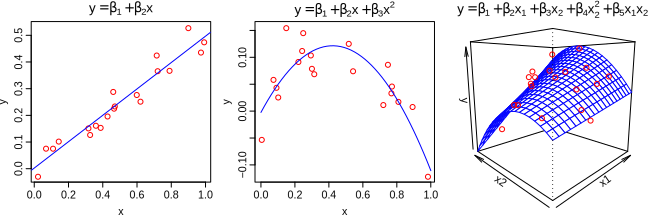
\includegraphics[width=.9\textwidth]{Linear.pdf}

	\item The data can be modelled (aka ``a mathematical model fitted to them'') as a {\it linear combination} of {\it variables} and {\it coefficients}
	\item Easily fitted using {\it Ordinary Least Squares} (OLS)
	\item Linear models can {\it include curved responses} (e.g. Polynomial regression)
\end{itemize}

% \begin{center} 
% 	{\tiny \href{https://www.mentimeter.com/s/befa8dbb37e8d1b0798e5f4669b40b67/1ba91b05de7a}{[link]}}

% 	\vspace{10pt}
% 	{\it Go to \url{www.menti.com} and enter code shown (phone or laptop)}
%   \vspace{10pt}
% \end{center}
\end{frame}


% %%%%%%%%%%%%%%%%%%%%%%%%%%%%%%%%%%%%%%%%%%%%%%%%%%%%%%
\begin{frame}{What makes a model non-linear?}

\begin{itemize}[<+->]\itemsep10pt

	\item OLS can be used to fit (model) equations that are {\it intrinsically linear},
	e.g.,
	\begin{itemize}
		\item 	Straight line: $y_i = \beta_0 + \beta_1 x_i + \varepsilon_i$
		\item Polynomial (quadratic): $y_i = \beta_0 + \beta_1 x_i + \beta_2 x_i^2 + \varepsilon_i$
		\item Another quadratic: $y_i = e^{\beta_0} + \beta_1 x_i + \beta_2 x_i^2 + \varepsilon_i$
	\end{itemize} 	
	\item What is {\it intrinsic linearity}? --- 
	the equation of the model to be fitted should be a {\it sum} of {\it linear terms}, i.e., the combination of {\it coefficient} (one of the $\beta$'s) and {\it variables} (the $x_i$'s):
	\item Some non-linear models:  
	\begin{itemize}
		\item $y_i = \beta_0 x_i^{\beta_1} + \varepsilon_i$
		\item $y_i = \beta_0 + \beta_1 x_i^{\beta_2} + \varepsilon_i$
		\item $y_i = \beta_0 e^{\beta_2 x_i} + \varepsilon_i$
		\item $y_i = \frac{\beta_0 x_i}{\beta_1 + x_i} + \varepsilon_i$
	\end{itemize}
	\pause In all of these, at least one term is non-linear (e.g., $x_i^{\beta_2}$, $e^{\beta_2 x_i}$, etc.) 
		
\end{itemize}

\end{frame}

%%%%%%%%%%%%%%%%%%%%%%%%%%%%%%%%%%%%%%%%%%%%%%%%%%%%%%
\begin{frame}{The Least-Squares Solution}

{\bf Recall what the Least Squares method does:}

	\begin{itemize}[<+->] \itemsep10pt

		\item Consider data on a response variable $y$, a predictor (independent) variable $x$, and $n$ observations. 
		
		\item Say we want to fit a model to these data: $
		f(x_i,\boldsymbol\beta) + \varepsilon_i $ 
		($\boldsymbol\beta = (\beta_0, \beta_1, \ldots,\beta_k)$ are 
		the model's $k+1$ parameters) 
		
		\item An example of $f(x_i,\boldsymbol\beta) + \varepsilon_i $ could be:
		$y_i = \beta_0 + \beta_1 x_i + \varepsilon_i$ (linear regression)

		\item The objective of any {\it least squares} method is to find estimates of values of the parameters ($\hat{\beta_j}$) that {\it minimize} the sum ($S$) of squared residuals ($r_i$) (AKA RSS):
		
		$$
		\text{RSS} = S = \sum\nolimits_{i=1}^n{\left[ y_i - f(x_i,\boldsymbol\beta) 
		\right]^2} = \sum\nolimits_{i=1}^n{r_i^2}
		$$
	
	\end{itemize}

\end{frame}

%%%%%%%%%%%%%%%%%%%%%%%%%%%%%%%%%%%%%%%%%%%%%%%%%%%%%%
\begin{frame}{The Least-Squares Solution}

	\begin{itemize}[<+->] \itemsep20pt

		\item The objective of any {\it least squares} method  is to find estimates of values of the parameters ($\hat{\beta_j}$) that minimize the sum ($S$) of squared residuals ($r_i$) (AKA RSS):
		
		$$
		\text{RSS} = S = \sum\nolimits_{i=1}^n{\left[ y_i - f(x_i,\boldsymbol\beta) 
		\right]^2} = \sum\nolimits_{i=1}^n{r_i^2}
		$$
		
		\item Let's picture this using a simple (OLS) example; fitting the model $y_i  = \beta_0 + \beta_1 x_i  +\varepsilon_i$...

	\end{itemize}

	
	% \begin{columns}[T]
	% \column{\textwidth}
	% 	\animategraphics[width=\textwidth, controls, buttonsize=1em, %timeline=Varying_timeline.txt % does not work - TODO
	% 	]{10}{Varying}{}{}
	% \end{columns}
	
	\end{frame}

	{
	\setbeamercolor{background canvas}{bg=}
	\includepdf[pages=1-50]{Varying.pdf}
	}	
%%%%%%%%%%%%%%%%%%%%%%%%%%%%%%%%%%%%%%%%%%%%%%%%%%%%%%
\begin{frame}{If the model is linear, the Least-Square solution is exact}
	
\begin{columns}[T]

	\column{0.5\textwidth}
		\includegraphics[width=\textwidth]{JustRight.pdf}
		
	\column{0.5\textwidth}
		\begin{align*}
		  y_i  & = \beta_0 + \beta_1 x_i  + {\color{red} \varepsilon_i }\\
		  \\
		  9.50  &= 5 + 4 \times 1 + {\color{red} 0.50}\\
		  11.00 &= 5 + 4 \times 2 - {\color{red} 2.00}\\
		  19.58 &= 5 + 4 \times 3 + {\color{red} 2.58}\\
		  20.00 &= 5 + 4 \times 4 - {\color{red} 1.00} 
		\end{align*}
		The least squares solution here is: $\beta_0 = 5; \beta_1 = 4$
				
\end{columns}		
\pause 
\begin{itemize}
	\item  \it This system of (linear) equations can be compactly represented (and solved using matrix algebra) as $\mathbf{Y} = \mathbf{X 
\boldsymbol\beta  +  \boldsymbol\varepsilon}$ 
\end{itemize}

\end{frame}

%%%%%%%%%%%%%%%%%%%%%%%%%%%%%%%%%%%%%%%%%%%%%%%%%%%%%%
\begin{frame}{Intrinsic non-linearity makes Least-Aquares model fitting difficult}

\begin{itemize}[<+->]\itemsep10pt

	\item In an {intrinsically non-linear model} such as $y_i = \beta_0
	e^{\beta_2 x_i} + \varepsilon_i$, the nice trick of solving  $\mathbf{Y} =
	\mathbf{X \boldsymbol\beta  + \boldsymbol\varepsilon}$ {\it exactly} is
	impossible	

\end{itemize}

\pause 
\begin{center}
	\includegraphics[width=.9\textwidth]{graphics/RSS_min.pdf}
\end{center}

\end{frame}

%%%%%%%%%%%%%%%%%%%%%%%%%%%%%%%%%%%%%%%%%%%%%%%%%%%%%%
\begin{frame}{OK, fine, why would {\it I} ever need NLLS?}

	\begin{itemize}[<+->]\itemsep10pt
		\pause 
		\item Many observations in biology are just {\it not} well-fitted by a linear model
	
		\item That is, the underlying biological phenomena/phenomenon are not 
		well-described by a linear equation
		
		\item Examples:
	
		\begin{itemize}\itemsep2pt
		
			\item Michaelis-Menten biochemical (reaction) kinetics
			
			\item Allometric growth
		
			\item Responses of metabolic rates to changing temperature 
	
			\item Consumer-Resource (e.g., predator-prey) functional responses 
			
			\item Individual growth
	
			\item Population growth
	
			\item Time-series data (e.g., fitting a sinusoidal function)
				
		\end{itemize}
	
		\item \it Can you think of some examples? 
	
	\end{itemize}
	
\end{frame}
	
%%%%%%%%%%%%%%%%%%%%%%%%%%%%%%%%%%%%%%%%%%%%%%%%%%%%%
\begin{frame}{Non-Linear Model Example: Temperature and metabolism}
		  
	\begin{columns}[c]
	  \column{2.1in}
	    \pause
	      \includegraphics[width=\textwidth]{graphics/Photobacterium.pdf}
	  \pause
	  \column{2.7in}
	    $B = B_0 \boxed {e^{-\frac{E}{kT}}}f(T,T_{pk},E_D)$\\
	    \vspace{10pt}
	    \raggedright{$T$ = temperature (K)\\
	     $k$ = Boltzmann constant (eV K$^{-1}$)}\\
	     $E$ = Activation energy (eV)\\
	     $T_{pk}$ = Temperature of peak performance\\
	     $E_D$ = Deactivation energy (eV)\\
	    {\small (J H van’t Hoff 1884, S Arrhenius 1889)}
	\end{columns}
	 
\end{frame}
	
	%%%%%%%%%%%%%%%%%%%%%%%%%%%%%%%%%%%%%%%%%%%%%%%%%%%%%%
	% \begin{frame}{Example: Functional responses}
	 
	% \begin{columns}[c]
	%   \column{2in}
	%   \begin{center}
	% 			   $f(x_R) = \frac{{a x_R^{q + 1}}}{{1 + h a x_R^{q + 1}}}$
	% 	\scriptsize (Holling, 1959)
	% 	\end{center}
	%  \scriptsize
	%  $x_R$ = Resource density (Mass / Area or Volume)\\
	%  $a$ = Search rate (Area or Volume / Time )\\
	%  $h$ = Handling time \\
	%  $q$ = Shape parameter (dimensionless) 
	%  \column{2.3in}
	%       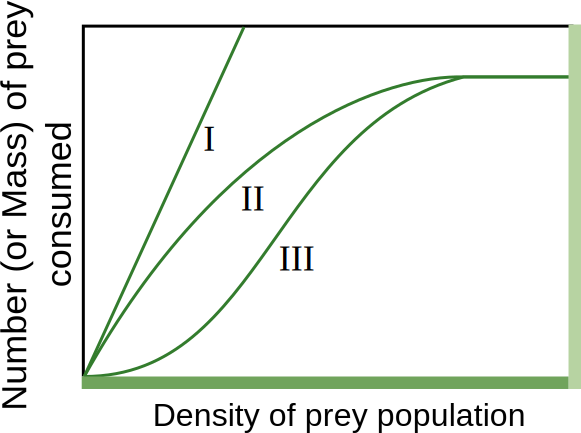
\includegraphics[width=\textwidth]{graphics/FR.pdf}
	% \end{columns}
	
	% \vspace{10pt}
	%  Note that: 
	% \begin{itemize}
	% \item NLLS fitting can yield $h < 0$, $q < 0$, or both 
	% \item $h < 0$ is biologically impossible but indicates an upward curving response
	% \item $q < 0$ is biologically unlikely as it indicates a decline in 
	% search rate with resource density (but is useful as a measure of 
	% deviation away from a type III response) 
	% \end{itemize}
	
	% \end{frame}
	
%%%%%%%%%%%%%%%%%%%%%%%%%%%%%%%%%%%%%%%%%%%%%%%%%%%%%%
\begin{frame}[plain]
 
	\begin{center}\LARGE 
		\textsc{The NLLS Fitting Method}
	\end{center}

\end{frame}

%%%%%%%%%%%%%%%%%%%%%%%%%%%%%%%%%%%%%%%%%%%%%%%%%%%%%%
\begin{frame}{The NLLS method: Overview}

	\begin{itemize}[<+->]\itemsep10pt
			
		\item OK, so we cannot find an exact, simple solution to the least-squares problem for non-linear models    
		
		\item But we can use a computer to find a {\it approximate but close-to-optimal} least-squares solution as follows:
		
		\begin{itemize}[<+->]\itemsep6pt
			\item Choose starting (initial values for the parameters we want to estimate ( $\beta_j$'s)
		
			\item Then, adjust the parameters {\it iteratively} (using a specific ``algorithm'' that is better than searching {\it randomly}) such that the RSS is gradually decreased 
	
			\item Eventually, if it all goes well, a combination of
		$\beta_j$'s that is {\it very close} to the desired solution (where the RSS is {\it approximately} minimized) can be found
				
		\end{itemize}
	\end{itemize}
	
	\end{frame}
	
%%%%%%%%%%%%%%%%%%%%%%%%%%%%%%%%%%%%%%%%%%%%%%%%%%%%%%
\begin{frame}{The NLLS fitting / optimization process}

	\begin{center}
		\includegraphics[width=\textwidth]{graphics/RSS_min.pdf}
	\end{center}

\end{frame}


%%%%%%%%%%%%%%%%%%%%%%%%%%%%%%%%%%%%%%%%%%%%%%%%%%%%%%

\begin{frame}{The NLLS fitting / optimization process}

The general procedure / algorithm is:

\begin{enumerate}[<+->] \itemsep4pt
	\item Start with an initial value for each parameter in the model
	\item Generate the curve defined by the initial values
	\item Calculate the residual sum-of-squares (RSS)
	\item Adjust the parameters to make the curve come closer to the data 
	points. {\it This the tricky part --- more on this in the next slide}
	\item Adjust the parameters again so that the curve comes even closer 
	to the points (RSS decreases)
	\item Repeat 4--5
	\item Stop simulations when the adjustments make virtually no 
	difference to the RSS
\end{enumerate}


\end{frame}

%%%%%%%%%%%%%%%%%%%%%%%%%%%%%%%%%%%%%%%%%%%%%%%%%%%%%%

\begin{frame}{NLLS fitting / optimization algorithms}

The {\it tricky part --- adjust parameters to make curve come closer to 
the data points} (step 4) --- has two main algorithms that are generally used:

\begin{itemize}[<+->]\itemsep10pt

	\item The {\bf Gauss-Newton} algorithm is often used, but doesn't work very well if the model to be fitted is mathematically complicated (the parameter search ``landscape'' is difficult) and the {\it starting values} for parameters are far-off-optimal
	
	\item The {\bf Levenberg-Marquardt} algorithm switches between
	Gauss-Newton and ``gradient descent'' and is more robust against starting
	values that are far-off-optimal and is more reliable in most scenarios.  
	
\end{itemize}   

\end{frame}

%%%%%%%%%%%%%%%%%%%%%%%%%%%%%%%%%%%%%%%%%%%%%%%%%%%%%%
\begin{frame}{NLLS fits -- assessment and reporting}

\begin{itemize}[<+->] \itemsep6pt
\item Once the NLLS fitting is done, you need to get the {\it goodness of fit measures}

\item First, of course, examine the fits visually

\item Report the goodness-fit results:

	\begin{itemize}
	
		\item Sums of deviations of the data points from the final model 
		fit (final RSS)
		\item Estimated coefficients
		\item For each coefficient, standard error (can be used for CI's), t-statistic and corresponding (two-tailed) p-value 
	\end{itemize} 

\item You will learn to calculate all these in the practicals   

\item You may also want to {\it compare and select between multiple competing  models}  

\item Unlike in Linear Models, R$^2$ values {\it should not} be used to interpret the quality of a NLLS fit (more on this in the practicals).    

\end{itemize}

\end{frame}

%%%%%%%%%%%%%%%%%%%%%%%%%%%%%%%%%%%%%%%%%%%%%%%%%%%%%%
\begin{frame}{NLLS Assumptions}

NLLS-regression has all the assumptions of OLS-regression:
	\begin{itemize}[<+->]\itemsep10pt
		
		\item No (in practice, minimal) measurement error in explanatory 
		variable ($x$-axis variable)
		
		\item Data have constant normal variance --- errors in the $y$-axis 
		are homogeneously distributed over the $x$-axis range
		
		\item The measurement/observation errors are Normally distributed (Gaussian) 
		% \pause 
		% --- for example, what would the error distribution of this 
		% non-linear model be: $y_i = \beta_0 e^{\beta_2 x_i} + 
		% \varepsilon_i$? \pause
		
		\item What if the errors are not normal? --- Interpret results
		cautiously, and use Maximum Likelihood or Bayesian fitting methods instead
	
	\end{itemize}
\end{frame}

%%%%%%%%%%%%%%%%%%%%%%%%%%%%%%%%%%%%%%%%%%%%%%%%%%%%%%
\begin{frame}[plain]
 
	\begin{center}\LARGE 
		\textsc{Practicals Overview}
	\end{center}

\end{frame}


%%%%%%%%%%%%%%%%%%%%%%%%%%%%%%%%%%%%%%%%%%%%%%%%%%%%%%

\begin{frame}{NLLS Fitting Practicals}
	
	\begin{itemize}[<+->]\itemsep16pt
	
		\item We will use {\tt R}
		
		\item For fitting simple non-linear models, the {\tt nls} function in R is sufficient 
			\begin{itemize}
				\item It uses the {\bf Gauss-Newton} algorithm by default
				\item The command is {\tt nls()}
				\item It is part of the {\tt stats} base package (so no extra installation and loading of package necessary)
			\end{itemize} 
			 
		\item For fitting complex non-linear models the {\bf Levenberg-Marquardt
		(LM)} algorithm is better

		\begin{itemize}
			\item The command is {\tt nlsLM()}
			\item It is available through the the {\tt minpack.lm} package {\small \url{http://cran.r-project.org/web/packages/minpack.lm}}
			\item It offers additional features like the ability to ``bound'' parameters to realistic values
		\end{itemize} 

	\end{itemize}   
	
	\end{frame}
	
%%%%%%%%%%%%%%%%%%%%%%%%%%%%%%%%%%%%%%%%%%%%%%%%%%%%%
\begin{frame}{NLLS Fitting Practicals}

\begin{itemize}\itemsep10pt

	\item We will start with NLLS fitting of the Michaelis-Menten model of biochemical reaction kinetics:

\end{itemize}
	
\begin{columns}[c]
	\column{.6\textwidth}
	\begin{center}
	$V = \frac{V_{\max}[S]}{K_{m} + [S]}$
	\end{center}

\begin{itemize} \scriptsize
	\item $S$ = Substrate density
	
		\item $V_{\max}$ = Maximum reaction rate (at saturating substrate concentration)
	
	\item $K_M$ = Half-saturation constant; the $S$ at which reaction rate reaches half of possible maximum ($=\frac{1}{2}V_{\max}$)
\end{itemize}
	
\column{.4\textwidth}
		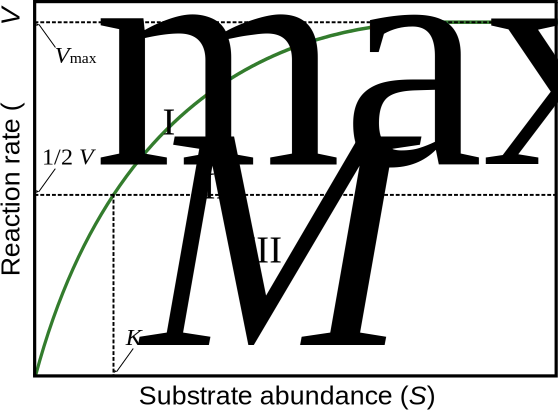
\includegraphics[width=\textwidth]{graphics/MM.pdf}
\end{columns}

\vspace{10pt}
\begin{itemize}\itemsep10pt

	\item You will use NLLS fitting to obtain estimates of $V_{\max}$ and $K_M$

	\item Note that $V_{\max} \le 0 $ and $K_M \le 0$ are physically impossible (useful fir picking starting values)

\end{itemize}

\end{frame}
	
%%%%%%%%%%%%%%%%%%%%%%%%%%%%%%%%%%%%%%%%%%%%%%%%%%%%%%

% \begin{frame}{More NLLS tips}

% \begin{itemize}[<+->]\itemsep10pt
% 	\item You can use mixed-effects modelling with NLLS in R; the package is {\tt nlme}
% 	{\small \url 
% 	{https://stat.ethz.ch/R-manual/R-devel/library/nlme/html/nlme.html}}
% 	(You are probably stuck with the Gauss-Newton algorithm with 
% 	{\tt nlme} though)
	
% 	\item You can also use Python --- look up {\tt lmfit} \url{https://lmfit.github.io/lmfit-py/index.html}. \\ {\tt python} seems to have a better Levenberg-Marqualdt implementation than {\tt R} 
	
% \end{itemize}   

% \end{frame}

%%%%%%%%%%%%%%%%%%%%%%%%%%%%%%%%%%%%%%%%%%%%%%%%%%%%%%

\begin{frame}{Readings}

\begin{itemize}\itemsep16pt
	
	\item Motulsky, Harvey, and Arthur Christopoulos. Fitting models to 	biological data using linear and nonlinear regression: a practical 
	guide to curve fitting. OUP USA, 2004. 
	
	% \item Johnson, J. B. \& Omland, K. S. 2004 Model selection in ecology and evolution. Trends Ecol. Evol. 19, 101--108. 

\end{itemize}   

\end{frame}

% %%%%%%%%%%%%%%%%%%%%%%%%%%%%%%%%%%%%%%%%%%%%%%%%%%%%%%
% \begin{frame}{Why is intrinsic non-linearity a problem?}

% % {\bf Let's use maths instead of brute-force computation!}

% 	\begin{itemize}[<+->] \itemsep16pt

% 		\item Our model is $f(x_i,\boldsymbol\beta) + \varepsilon_i$ \\ 
			
% 		\item We want to find estimates of values of the parameters 
% 		($\hat{\beta_j}$) that {\it minimize} the sum ($S$) of squared residuals 
% 		($r_i$) (AKA ``RSS'') $S = \sum\nolimits_{i=1}^n{\left[ y_i - 
% 		f(x_i,\boldsymbol\beta) \right]^2} = \sum\nolimits_{i=1}^n{r_i^2}$

% 		\item For this we can solve $\frac{\partial S}{\partial 
% 		\beta_j} = 0, j = 0,1,2,\ldots,k$ to find the {\it minimum}
	
% 		\item That is, we need to solve	
% 		$\frac{\partial \sum\nolimits_{i=1}^n{r_i^2}}{\partial \beta_j} = 
% 		0$
		
% 		\item Or, $2 \sum\nolimits_{i=1}^n r_i \frac{\partial r_i}{\partial \beta_j} = 0$
	
% 	\end{itemize}

% \end{frame}

% %%%%%%%%%%%%%%%%%%%%%%%%%%%%%%%%%%%%%%%%%%%%%%%%%%%%%%
% \begin{frame}{Why is intrinsic non-linearity a problem?}

% 	\begin{itemize}[<+->] \itemsep16pt

% 		\item Thus, solving $ 2 \sum\nolimits_{i=1}^n r_i \frac{\partial r_i}{\partial \beta_j} 
% 		= 0$ \\
		
% 		boils down to finding the ``gradient'' $ \frac{\partial r_i}{\partial \beta_j} $
	
% 		\item This is not a problem in linear models, because this gradient 
% 		is fully solvable as the equation is {\it intrinsically linear}
		
% 		\item That is, the solution of $ \frac{\partial r_i}{\partial 
% 		\beta_j} $ is simple (enough)  
				
% 	\end{itemize}

% \end{frame}

% %%%%%%%%%%%%%%%%%%%%%%%%%%%%%%%%%%%%%%%%%%%%%%%%%%%%%%
% \begin{frame}{Why is intrinsic non-linearity a problem?}

% 	\begin{itemize}[<+->] \itemsep16pt
		
% 		\item For example, if $f(x_i,\boldsymbol\beta) + \varepsilon_i = \beta_0 + \beta_1 x_i + 
% 		\varepsilon_i$ \\
		
% 		\item That is, our model is $y_i = \beta_0 + \beta_1 x_i + \varepsilon_i$ 
% 		(Linear Regression)
		
% 	\item Then we want to solve 
		
% 		$\frac{\partial S}{\partial {\beta_0}} = 
% 		\sum\nolimits_{i=1}^{n}{\frac{\partial {{\left[ 
% 		y_i-(\beta_0+\beta_1 x_i) \right]}^{2}}}{\partial {{\beta 
% 		}_{0}}}}=0 $ \\
		 
% 		$ \frac{\partial S}{\partial {{\beta 
% 		}_{1}}}=\sum\nolimits_{i=1}^{n}{\frac{\partial {{\left[ 
% 		{{y}_{i}}-({{\beta }_{0}}+{{\beta }_{1}}{{x}_{i}}) 
% 		\right]}^{2}}}{\partial {{\beta }_{1}}}} = 0$
		
% 	\end{itemize}

% \end{frame}

% %%%%%%%%%%%%%%%%%%%%%%%%%%%%%%%%%%%%%%%%%%%%%%%%%%%%%%
% \begin{frame}{Why is intrinsic non-linearity a problem?}

% 	\begin{itemize}[<+->] \itemsep16pt

% 		\item And, solving\\ 		
% 		$\frac{\partial S}{\partial {\beta_0}} = 
% 		\sum\nolimits_{i=1}^{n}{\frac{\partial {{\left[ 
% 		y_i-(\beta_0+\beta_1 x_i) \right]}^{2}}}{\partial {{\beta 
% 		}_{0}}}}=0 $\\ 
		 
% 		$ \frac{\partial S}{\partial {{\beta }_{1}}}=\sum\nolimits_{i=1}^{n}{\frac{\partial 
% 		{{\left[ {{y}_{i}}-({{\beta }_{0}}+{{\beta }_{1}}{{x}_{i}}) 
% 		\right]}^{2}}}{\partial {{\beta }_{1}}}} = 0$ \\
		
% 		\vspace{6pt}
% 		just boils down to solving two simultaneous equations because $ 
% 		\frac{\partial r_i}{\partial \beta_j} $ is simple {\it because} the model 
% 		is intrinsically linear:\\
		
% 		\vspace{6pt}
% 		$-n{{\beta }_{0}}+\sum\nolimits_{i=1}^{n}{{{y}_{i}}}+{{\beta 
% 		}_{1}}\sum\nolimits_{i=1}^{n}{{{x}_{i}}}=0 $\\ 
		
% 		$ \sum\nolimits_{i=1}^{n}{{{x}_{i}}{{y}_{i}}}-{{\beta 
% 		}_{0}}\sum\nolimits_{i=1}^{n}{{{x}_{i}}}+{{\beta 
% 		}_{1}}\sum\nolimits_{i=1}^{n}{x_{i}^{2}}=0$

% 		\item That is, we need to solve $\mathbf{Y} = \mathbf{X 
% 		\boldsymbol\beta  +  \boldsymbol\varepsilon}$ ({\it this is what R 
% 		solves when you use {\tt lm()}})

% 	\end{itemize}

% \end{frame}


%%%%%%%%%%%%%%%%%%%%%%%%%%%%%%%%%%%%%%%%%%%%%%%%%%%%%%
\end{document}
